\documentclass[Main.tex]{subfiles} 
\begin{document}

\subsubsection{Use Case 1.2: Bestem materialetype realisering}

Use Case 1.2 "Bestem materialetype" er opbygget ved at system har noget data fra forrige Use Case (UC 1.1 - M�l og vej klods) der udregnes til en bestemt densitet i Business logic layer. Derefter kalder systemet ned i Data access layer, hvor kommunikationen til databasen findes. Her sammenlignes den udregnede densitet med den persisterede densitet. Derudfra kan materialetypen bestemmes og Use Casen er udf�rt samt udfyldt.

Interaktionsdiagram over "Bestem materialetype":
\begin{figure}[H]
	\centering
	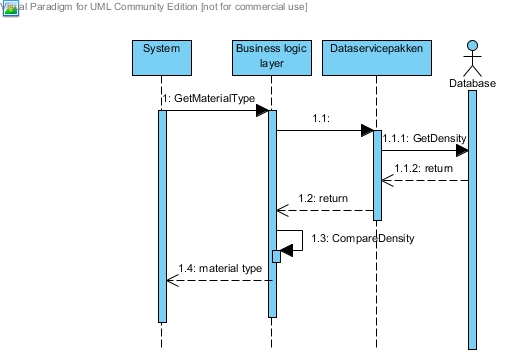
\includegraphics[scale=0.75, trim = 30mm 0mm 0mm 10mm, clip]{./Diagrammer/SSD/5_3_3_Use_Case_1_2_Bestem_materialetype_realisering.jpg}
	\caption{Simpelt sekvensdiagram af bestem materialetype}
	\label{fig:5_3_3_Use_Case_1_2_Bestem_materialetype_realisering}
\end{figure}



\end{document}